% \chapter{CONSIDERAÇÕES FINAIS}



% O teste de software é um processo custoso e que demanda muitos recursos e tempo para ser planejado e executado, porém é parte fundamental no desenvolvimento de sistemas que buscam por qualidade.  O principal objetivo do presente trabalho é cobrir totalmente os testes de unidade e testes de componentes do sistema MIP, buscando a verificação e validação dos requisitos coletados promovendo uma melhoria do sistema como um todo. Estas etapas são apenas o início de um plano de teste de software. Ainda restam outras etapas que devem ser implementadas como o teste de sistema e teste de aceitação que não serão tratados neste trabalho e devem ser explorados em trabalhos futuros. 

\chapter{DESENVOLVIMENTO}


\section{CONFIGURAÇÕES INICIAIS}

\subsection{Estrutura do Projeto}



A estrutura de diretórios gerados pelo \textit{framework Spring Boot} garante a divisão do código fonte, promovendo a separação das classes e suas responsabilidades. Além disso é possível adotar uma subestrutura, está deve seguir um padrão arquitetural mantendo a organização e facilitando a manutenção do projeto. A FIGURA \ref{estruturaProjeto} apresenta o estado atual do projeto e suas divisões em diretórios e subdiretório. 


\begin{figure}[H]
	\centering
	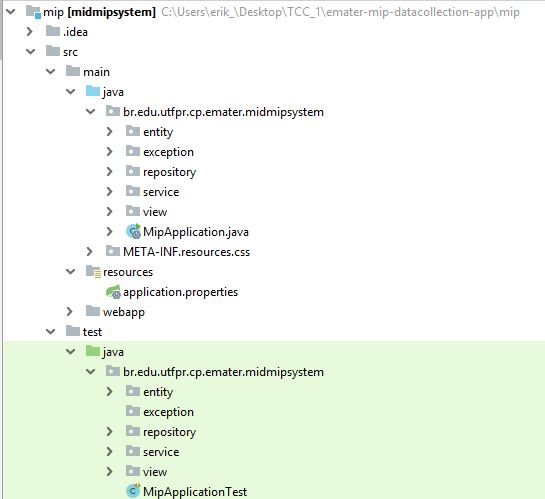
\includegraphics[]{dados/figuras/estruturaDoProjeto.JPG}
	\caption{Estrutura do projeto \textit{Spring Boot.}}
	\label{estruturaProjeto}
\end{figure}

    Um diretório pode conter nenhum, um ou mais de um subdiretório ou classes dentro dele. O projeto apresentado na FIGURA \ref{estruturaProjeto}  segue o padrão de nomenclatura especificado  pela convenção de código Java publicado pela \textit{Sun} e mantida pela \textit{Oracle} \cite{Oracle}, juntamente de diretórios pré-configurados pelo \textit{Spring-Boot} e pelo \textit{Maven} o que permite a familiarização imediata de novos usuários que já utilizaram o \textit{framework.} Estes diretórios possuem o seguinte contexto: 



\begin{itemize}
    \item \textbf{src/main/java:} Diretório onde está o código fonte Java da Aplicação.
\item \textbf{src/main/META-INF.resources.css:} Diretório usado para configurar informações de metadados do projeto, geralmente dados web como folhas de estilo CSS.
\item \textbf{src/main/resources:} Arquivos de configuração e outros arquivos devem ficar nesta pasta.
\item \textbf{src/main/webapp:} Diretório para conteúdo Web. Aqui se encontra todos os arquivos fonte da parte web.
\item \textbf{src/test/java:} Diretório que contém os arquivos de testes unitários.
\item \textbf{src/test/resources:} Diretório com arquivos que serão utilizados pelas classes de testes unitários
\end{itemize}


O padrão da \textit{Sun} utilizado para dar nome aos subdiretórios é relativo ao nome da instituição em que o projeto é desenvolvido:

\begin{itemize}
 
\item \textbf{br/edu/utfpr/cp/emater/midmipsystem/}
\end{itemize}


Os diretório só possuem letras minúsculas, não importa quantas palavras estejam contidas nele. Esse padrão existe para evitar ao máximo o conflito de diretório de instituições diferentes.

Os subdiretórios representam a divisão arquitetural em camadas do sistema onde cada diretório possui a seguinte responsabilidade: 

\begin{itemize}
 

\item \textbf{Entity (Domínio):} Implementa entidades, interfaces para serviços, validações e classes do domínio. 


\item \textbf{Repository (Infraestrutura):} Implementa a persistência dos dados e os repositórios.

\item \textbf{Service (Serviços):} Implementa a comunicação da aplicação com a interface.

\item \textbf{View (Apresentação):} Implementa a interface do usuário.

\item \textbf{Exception:} Implementa o tratamento de erros específicos que podem acontecer durante execução da aplicação.
\end{itemize}

O diretório de \textit{test} segue o modelo estrutural do diretório main e seus subdiretórios, mais por convenção toda classe do diretório de teste deve seguir o padrão: classe+Test. O que proporciona a identificação e a separação das classes de testes.  

\subsection{Controle de versão}

Para realizar o controle de versão do projeto será utilizado o \textit{Git} na máquina local e o \textit{Github} como repositório remoto. O \textit{Github} possibilita que uma equipe de desenvolvimento trabalhe de forma centralizada e organizada auxiliando a manter o histórico de alterações do projeto permitindo ao administrador controlar o que é alterado, quando foi alterado e qual usuário alterou, possibilitando a voltar a uma versão mais estável caso uma alteração gere uma inconsistência.

 Por se tratar de um trabalho colaborativo o repositório do projeto já estava criado no endereço: \textit{https://github.com/gabrielcostasilva/emater-mip-datacollection-app}, porem para que as alterações não fossem realizadas diretamente no projeto original podendo gerar erros, foi feito um clone da versão original gerando um novo repositório no endereço: \textit{https://github.com/ErikZA/emater-mip-datacollection-app}. Posteriormente as alterações feitas no projeto clonado podem ser enviadas ao repositório original através de um \textit{pull request}\footnote{Pull Request é quando se envia uma sugestão de melhoria para o repositório.}. O administrador avaliará as alterações, depois da análise de impacto ele deve aceitá-las ou recusá-las.




\subsection{Controle do projeto}

O \textit{Github} também oferece diversas ferramentas para melhorar o controle do projeto. Depois de criar ou clonar um repositório é possível adicionar tarefas que devem ser resolvidas chamadas de \textit{"issues”} pelo \textit{Github}. Estas \textit{issues} podem receber diferentes etiquetas de acordo com o impacto que elas têm no projeto. A FIGURA \ref{issues} apresenta as \textit{issues} que foram criadas para este projeto assim como a etiqueta que cada uma delas recebeu de acordo com o seu impacto:

\begin{figure}[H]
	\centering
	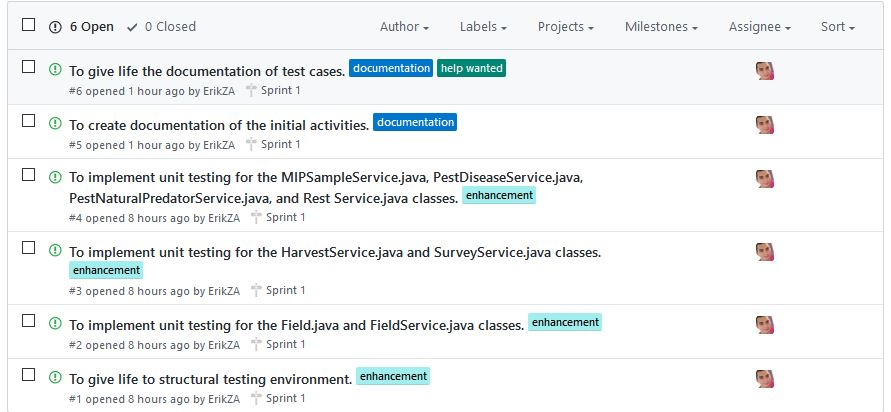
\includegraphics[scale=0.7]{dados/figuras/issues.JPG}
	\caption{\textit{Issues} do projeto.}
	\label{issues}
\end{figure}


As \textit{issues} listadas na FIGURA \ref{issues} tem as seguintes funções:


\begin{itemize}
 \item[1] \textit{To give life to structural testing environment. Label: enhancement (New feature or request)}\footnote{Para dar vida ao ambiente de testes estruturais. Etiqueta: valorização (novo recurso ou pedido)}

\item \textit{It consists of adding the necessary dependencies and creating the structure of folders that allow the execution of the unit tests.}\footnote{Consiste em adicionar as dependências necessárias e criar a estrutura das pastas que permitem a execução dos testes unitários.}

 \item[2] \textit{To implement unit testing for the Field.java and FieldService.java classes. Label: enhancement (new feature or request)}\footnote{Para implementar testes de unidade para as classes Field.java e FieldService.java. Etiqueta: valorização (novo recurso ou pedido)}

\item \textit{Consist on testing the Field.java and FieldService.java classes.}\footnote{Consistem em testar as classes Field.java e FieldService.java.}

 \item[3] \textit{To implement unit testing for the HarvestService.java and SurveyService.java classes. Label: enhancement (new feature or request)}\footnote{Para implementar testes de unidade para as classes HarvestService.java e SurveyService.java. Etiqueta: valorização (novo recurso ou pedido)}

\item \textit{Consist on testing the HarvestService.java and SurveyService.java classes.}\footnote{Consistem em testar as classes HarvestService.java e SurveyService.java.}

 \item[4] \textit{To implement unit testing for the MIPSampleService.java, PestDiseaseService.java, PestNaturalPredatorService.java, and Rest Service.java classes. Label: enhancement (new feature or request)}\footnote{Para implementar testes de unidade para as classes MIPSampleService.java, PestDiseaseService.java, PestNaturalPredatorService.java e Rest Service.java. Etiqueta: valorização (novo recurso ou pedido)}

\item \textit{Consist of testing the MIPSampleService.java, PestDiseaseService.java, PestNaturalPredatorService.java, and PestService.java.}\footnote{Consiste em testar o MIPSampleService.java, o PestDiseaseService.java, o PestNaturalPredatorService.java e o PestService.java.}


 \item[5] \textit{To create documentation of the initial activities. Label: Documentation (Improvements or additions to documentation)}\footnote{
Para criar documentação das atividades iniciais. Etiqueta: documentação (melhorias ou adições a documentação)}

\item \textit{Preparation of the tcc2 document.}\footnote{Elaboração do documento tcc2.}

 \item[6] \textit{To give life the documentation of test cases. Documentation (Improvements or additions to documentation), label: help wanted (Extra caution is required)}\footnote{Para dar vida a documentação dos casos de teste. Etiqueta: documentação (melhorias ou adições a documentação), etiqueta: Procura-se ajuda (é necessária cautela Extra)}
 
\item \textit{Create documentation of the initial activities. Flow Graph Notation. Cyclomatic Complexity. Derivation of Test Cases.}\footnote{Notação de Fluxograma. Complexidade ciclomática. Derivação de Casos de Teste.}

\end{itemize}{}




Além disso e possível marcar uma data no projeto chamado no Github de “Milestones”, esta marcação foi utilizada de forma a estipular uma data de conclusão de um determinado conjunto de issues do projeto, é possível associar está marcação as issues facilitando o controle e o monitoramento do projeto. A FIGURA \ref{splint1} apresenta os milestones criados para o projeto: 
\begin{figure}[H]
	\centering
	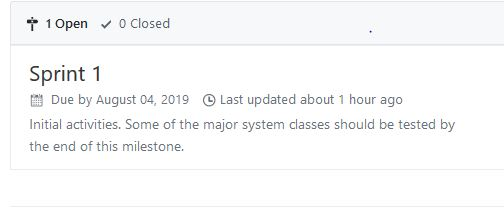
\includegraphics[scale=1.1]{dados/figuras/milestones.JPG}
	\caption{Marco para o primeiro Sprint.}
	\label{splint1}
\end{figure}

Cada milestones representa a entrega de um conjunto de funcionalidades do projeto, cada entrega foi definida da seguinte forma:

\begin{itemize}
    \item[1]\textit{\textbf{Sprint 1} Initial activities. Some of the major system classes should be tested by the end of this milestone.}\footnote{Atividades iniciais. Algumas das principais classes do sistema devem ser testadas até o final desse marco.}
    \item \textit{Due by August 04, 2019}\footnote{ Entrega até 04 de agosto de 2019}
\end{itemize}{}

Após criar as \textit{issues} e os \textit{milestone} é possível associá-los a um \textit{Github projects}, que permite criar fases de execução do projeto. Esta ferramenta permite controlar a execução das issues atribuindo-as a uma fase dentro do projeto.  A FIGURA \ref{controleAtividades} apresenta o controle da execução das \textit{issues} e as fases do projeto:

A FIGURA \ref{controleAtividades} apresenta o projeto, suas fases e a posição de cada \textit{issues} dentro do projeto.   O projeto possui 4 fases: \textit{To do} (Façam); \textit{In progress} (Em progresso); \textit{In revision} (Em revisão); \textit{Done} (Feito). Uma nova \textit{issue} deve entrar no projeto na fase \textit{To do}, esta fase indica que a tarefa ainda deve ser realizada. Quando a issue seguir para produção ela deve passar para a fase \textit{in progress}, o que indica que a atividade esta sendo realizada. Posteriormente esta atividade deve ser apresentada e revisada ao final de cada \textit{milestones}, está fase é a \textit{In revision}. Após a apresentação e validação das atividades executadas a atividade é direcionada a fase \textit{Done}, o que encerra a \textit{issue}.
\begin{landscape}
\begin{figure}[H]
	\centering
	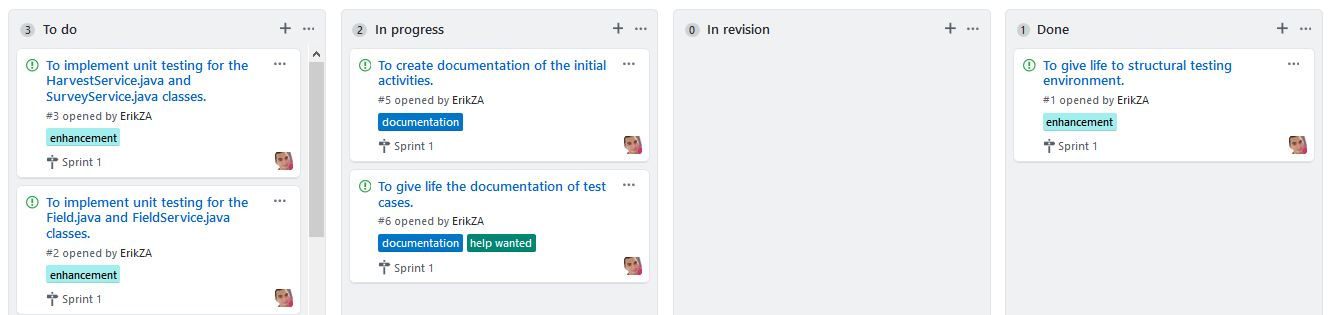
\includegraphics[scale=0.7]{dados/figuras/atividadesProjeto.JPG}
	\caption{Controle das atividade.}
	\label{controleAtividades}
\end{figure}
\end{landscape}



\section{LIÇÕES APRENDIDAS}

\begin{itemize}
    \item Uma das diferenças da faculdade para um projeto de trabalho real é que o curso superior te prepara para uma área de conhecimento, o que dá ao aluno um conhecimento muito mais teórico. Enquanto projetos de trabalho exigem uma formação muito mais técnica e um profundo conhecimento de ferramentas e frameworks que oferecem um conjunto de funcionalidades prontas, o que torna a teoria pouco eficiente nestes casos pois o projeto exige produtividade.
    
    \item A defasagem de muitos cursos é um problema, a universidade tenta construir uma base solida de conhecimento para cada aluno, mas muitos cursos estão desatualizados ou acabam não atingindo o objetivo por falta de carga horaria ou ementa desatualizada. O fato é que a tecnologia se atualiza muito rápido é muito do que é ensinado ainda é muito básico para o mercado que em sua maioria exige profissionais que conheçam as mais novas tecnologias. Talvez a burocracia publica atrapalhe a UTFPR neste ponto.
    
    \item O mercado de trabalho está muito exigente o que torna um profissional graduado pouco relevante, a falta de certificações técnicas oficias faz falta na formação pois certificações JAVA ou outras ajudariam no desenvolvimento de projetos e na formação do profissional.
    
\end{itemize}{}



% \chapter{EQUAÇÕES}

% \chapter{SOBRE AS LISTAS}

% \chapter{SOBRE AS CITAÇÕES E CHAMADAS DE REFERÊNCAS}



